\chapter{Random(Erase)}

\graphicspath{{./Figures/Design}}

This comprehensive chapter unfolds the intricate details of the new design of our two-wheeled self-balancing robot, an advanced piece of engineering that incorporates additional degrees of freedom to enhance its movement capabilities. Through an exploration of the various motions the robot can perform, we delve into the intricate design considerations of each component, ensuring that they align with the overall functional and aesthetic vision. 


\begin{figure}[h]
	\centering
	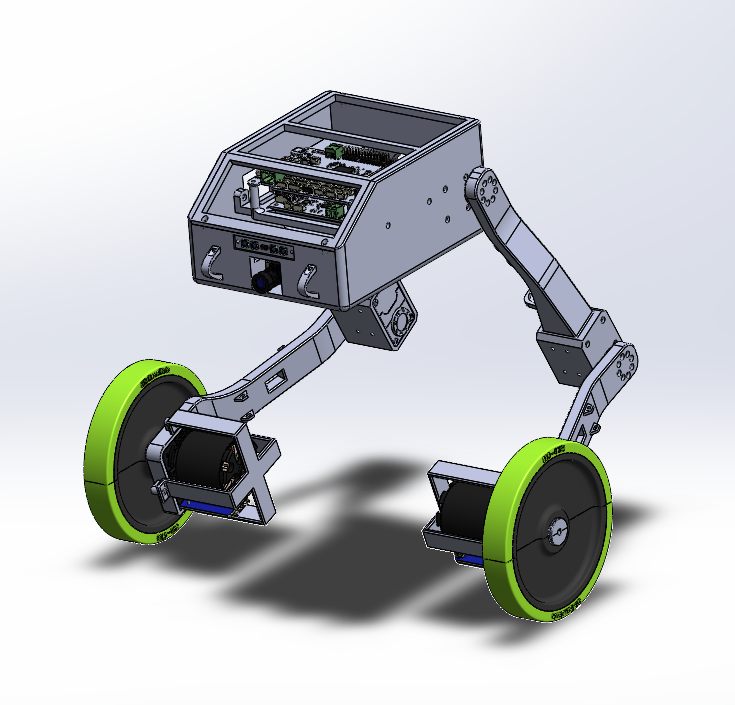
\includegraphics[width=1\textwidth]{/Capture}
	\caption[Moment of inertia Schematic representation]{Schematic representation detailing the requisite angles and lengths for calculating the moment of inertia.}
	\label{fig:Schematic representation detailing the requisite angles and lengths for calculating the moment of inertia.}
\end{figure}
\newpage
\begin{itemize}
	\item The Robot new design.
	\item The added degrees of freedom.
	\item Different motions that can be performed.
	\item Discussing each component of the robot and things taken into account while designing it.
	\begin{itemize}
		\item Body
		\begin{itemize}
		\item overall design inspiration
		\item For the body: the consideration for including all the necessary components in a compact form is to optimize the use of space and at the same time distribute the weight equally.
		\item The body includes the hip motors, the battery, camera, sensor, a rack that includes the motors drivers board, the micro-controller board attached to the Raspberry Pi.
		\item fastening features that were specifically designed in order to easily mount the battery, organize the cable between the boards and the rest of the robot parts.
		\item Features for modular design and easy printing.
		\end{itemize}
			\item Thigh
		\begin{itemize}
			\item curvature of that joint to give room for the motors 
			\item cable management 
			\item motor cover to insure its fixation. 
		\end{itemize}
			\item Calf
		\begin{itemize}
			\item curvature of that joint and the thigh joint combined make enough room for the wheel motor so the it have clearance from the body. 
			\item cable management 
			\item motor mount and additional frame.
		\end{itemize}
	\end{itemize}
\end{itemize}





\newpage


\begin{figure}[h]
	\centering
	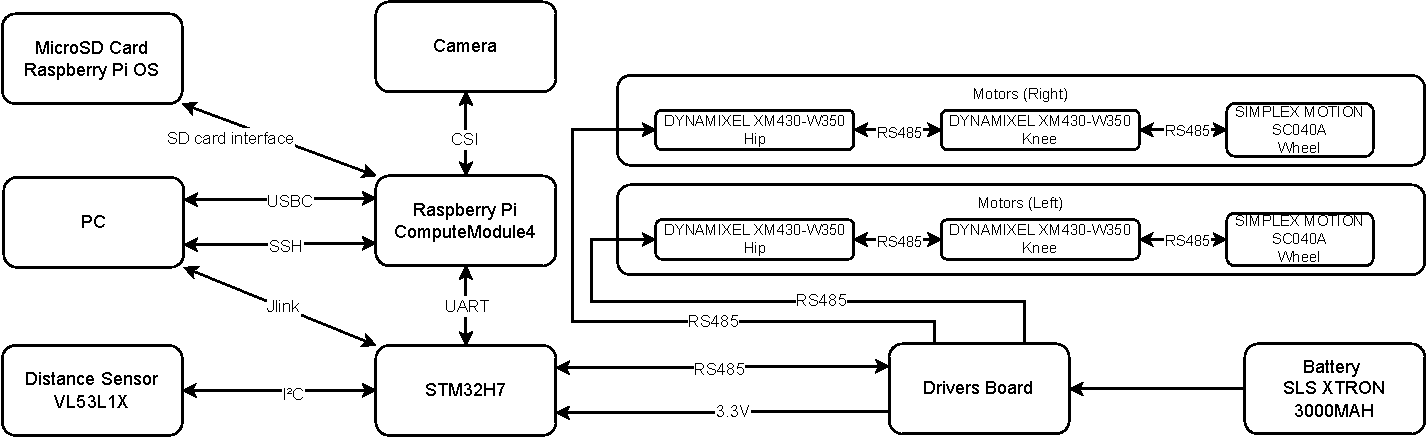
\includegraphics[width=1\textwidth]{/Component_diagram.pdf}
	\caption[Moment of inertia Schematic representation]{Schematic representation detailing the requisite angles and lengths for calculating the moment of inertia.}
	\label{fig:Schematic representation detailing the requisite angles and lengths for calculating the moment of inertia.}
\end{figure}
\begin{itemize}
	\item electronic components 
	\begin{itemize}
		\item Motors taking into count the needed torque and speed
		\item comparison between the BLDC and Geared Robotic 
		\item RS-485 communications protocol compared to others 
		\begin{itemize}
			\item for the knee and hip motors high torque and low speed is needed.(calculations the show the weights and the needed torques)
			\item for the wheel motors high speed and low torque is needed. 
		\end{itemize}
		\item Boards 
		\begin{itemize}
			\item STM high performance h7 constum board connected with rasberrypi 
			\item driver board that provide the power for 6 motors. 
		\end{itemize}
		\item modules 
		\begin{itemize}
			\item camera module.
			\item distance sensor.
		\end{itemize}
	\end{itemize}
\end{itemize}



